\documentclass[12pt]{article}
\usepackage[LGR, T1]{fontenc}
\usepackage[utf8]{inputenc}
\usepackage[greek,english]{babel}
\usepackage{alphabeta}
\usepackage{multicol}
\usepackage[margin=0.8in]{geometry}
\usepackage{microtype}
\usepackage{csvsimple}
\usepackage{multirow}
\usepackage{graphicx}
\usepackage{tikz}
\usepackage{hyperref}
\usepackage{algorithm} 
\usepackage{algorithmic}
\usepackage{csquotes}
\usepackage{amsmath}
\usepackage{amssymb}
\usepackage{alphabeta}
\usepackage{pgfgantt}
\usepackage{xcolor}  
\usepackage{framed}
\usepackage{listings}
\usepackage{tabularx}
\usepackage{adjustbox}
\usepackage{caption}
\usepackage{minted}
\usepackage{cite}
\usepackage{pifont}
\usepackage{textcomp}
\usepackage{subfigure}
\usepackage{subcaption}
\usepackage{listings}


\title{Εργαστηριακή Άσκηση 3 \\ Scale Invariant Fetuare Transform (SIFT)}
\author{Μαριάνθη Θώδη}
\date{Δεκέμβριος 2025}

\begin{document}
\begin{figure}
\begin{flushleft}
  
\includegraphics[width=6cm]{logo.png}
  \hfill
\end{flushleft}
\end{figure}

\maketitle
\newpage
\tableofcontents

\section{Abstract}
Η παρούσα εργαστηριακή άσκηση εστιάζει στη μελέτη και υλοποίηση του αλγορίθμου SIFT, για την εξαγωγή χαρακτηριστικών. Σκοπός της άσκησης είναι η κατανόηση της διαδικασίας ανίχνευσης 
(keypoints) που παραμένουν αναλλοίωτα σε μετασχηματισμούς κλίμακας και περιστροφής. Η διαδικασία περιλαμβάνει τη δημιουργία χώρου κλίμακας (Scale Space) μέσω της διαφοράς γκαουσιανών (DoG), τον εντοπισμό τοπικών ακροτάτων και τη δημιουργία μοναδικών descriptors. 
Τέλος, εξετάζεται η αντιστοίχιση των χαρακτηριστικών μεταξύ διαφορετικών εικόνων και η βελτιστοποίηση των αποτελεσμάτων μέσω του αλγορίθμου RANSAC για την απόρριψη λανθασμένων αντιστοιχιών (outliers).
Ο πλήρης κώδικας και τα αρχεία της άσκησης διατίθενται σε repo στο GitHub στον αντίστοιχο σύνδεσμο \href{https://github.com/palpatinedude/Computer-Vision-.git}{GitHub Repository}.
\section{Αλγόριθμος SIFT}
Ο αλγόριθμος αυτός ανιχνεύει και περιγράφει interesting points σε εικόνες και εντοπίζει σταθερά χαρακτηριστικά σημεία (keypoints) τα οποία:
\begin{enumerate}
    \item Scale invariant 
    \item Rotation invariant
    \item Είναι ανθεκτικά σε μεταβολές φωτισμού και μικρές γεωμετρικές παραμορφώσεις
\end{enumerate}
Ο αλγόριθμος SIFT αποτελείται από 2 μέρη:
\begin{itemize}
    \item Ανιχνευτή (detector) σημείων ενδιαφέροντος
    \item Περιγραφέα (descriptor) των σημείων αυτών
\end{itemize}
Η βασική ιδέα του αλγορίθμου είναι η ανίχνευση ακρότατων στον χώρο κλίμακας της διαφοράς γκαουσιανών (DoG), 
η οποία αποτελεί προσέγγιση της κανονικοποιημένης λαπλασιανής (LoG).
\subsection{Τα Τέσσερα Στάδια του Αλγορίθμου SIFT}
Ο αλγόριθμος SIFT χωρίζεται σε τέσσερα βασικά στάδια, τα οποία παρουσιάζονται στη συνέχεια.

\subsection{Στάδιο 1 : Χώρος Κλίμακας \& DoG}
\paragraph{Scale Space}
\mbox{}\\
Ο χώρος κλίμακας μιας εικόνας ορίζεται ως:

\[
L(x,y,\sigma) = G(x,y,\sigma) * I(x,y)
\]

όπου:

\begin{itemize}
  \item $I(x,y)$: η αρχική εικόνα
  \item $G(x,y,\sigma)$: ο γκαουσιανός πυρήνας
  \item $\sigma$: η παράμετρος κλίμακας
\end{itemize}
Για την επίτευξη scale invariant, ο SIFT οργανώνει τον χώρο κλίμακας σε οκτάβες,
όπου κάθε οκτάβα αντιστοιχεί σε διπλασιασμό της κλίμακας(blur scale) και υποδειγματοληψία της εικόνας κατά παράγοντα 2.

\paragraph{Difference of Gaussians (DoG)}
\mbox{}\\
Η διαφορά γκαουσιανών ορίζεται ως:

\[
D(x,y,\sigma) = L(x,y,k\sigma) - L(x,y,\sigma)
\]

Η DoG αποτελεί μια προσέγγιση της κανονικοποιημένης λαπλασιανής:

\[
\mathrm{DoG} \approx (k - 1)\sigma^2 \nabla^2 L
\]

και επιτρέπει την ανίχνευση σημείων ενδιαφέροντος με μικρό υπολογιστικό κόστος διότι:
\begin{enumerate}
    \item η DoG υπολογίζεται ως αφαίρεση δύο ήδη φιλτραρισμένων εικόνων με γκαουσιανά φίλτρα.
    \item Τα gaussian φίλτρα είναι separable, γεγονός που μειώνει την πολυπλοκότητα των συνελίξεων.   
\end{enumerate}
Αντίθετα, η χρήση της LoG θα απαιτούσε:
\begin{enumerate}
    \item Υπολογισμό δευτέρων παραγώγων για κάθε επίπεδο κλίμακας
    \item Συνέλιξη της εικόνας με μη διαχωρίσιμα φίλτρα LoG
    \item Σημαντικά αυξημένο υπολογιστικό κόστος και μνήμης
\end{enumerate}
Με βάση τα παραπάνω καταλαβαίνουμε ότι τα ακρότατα της DoG συμπίπτουν με τα ακρότατα της NLoG .

\subsection{Στάδιο 2 : Ανίχνευση Τοπικών Ακρότατων}
Στο δεύτερο στάδιο του αλγορίθμου πραγματοποιείται η ανίχνευση τοπικών ακρότατων της συνάρτησης DoG στον χώρο κλίμακας. 
Το στάδιο αυτό ονομάζεται ανίχνευση σημείων ενδιαφέροντος και βασίζεται στη θεωρία της NLoG.

Σύμφωνα με τη θεωρία scale-space, τα σταθερά χαρακτηριστικά σημεία (blobs) αντιστοιχούν σε ακρότατα της ποσότητας:

\[
\sigma^2 \nabla^2 L(x,y,\sigma)
\]

η οποία προσεγγίζεται μέσω της διαφοράς γκαουσιανών όπως αναφέρθηκε παραπάνω. Για τον εντοπισμό αυτών των ακρότατων, κάθε εικονοστοιχείο της εικόνας DoG
συγκρίνεται με τα 26 γειτονικά εικονοστοιχεία του στον τρισδιάστατο χώρο $(x,y,\sigma)$:  
\begin{itemize}
    \item 8 γείτονες στην ίδια κλίμακα
    \item 9 στην προηγούμενη κλίμακα
    \item  9 στην επόμενη κλίμακα
\end{itemize}
Ένα σημείο χαρακτηρίζεται ως υποψήφιο σημείο-κλειδί (keypoint) αν η τιμή του είναι είτε αυστηρά μεγαλύτερη είτε αυστηρά μικρότερη
από όλες τις αντίστοιχες τιμές των γειτονικών του σημείων. Με αυτόν τον τρόπο εξασφαλίζεται ότι το σημείο αποτελεί τοπικό ακρότατο τόσο ως προς τη χωρική
θέση $(x,y)$ όσο και ως προς την κλίμακα $\sigma$.

\subsection{Στάδιο 3 : Φιλτράρισμα και Εντόπιση Keypoints}
Τα υποψήφια keypoints φιλτράρονται ώστε να παραμείνουν μόνο τα αξιόπιστα.Περιλαμβάνει τρία κύρια βήματα:
\paragraph{Υπο-πίξελ \& Υπο-κλίμακα Εντοπισμός}
\mbox{}\\
Κάθε υποψήφιο keypoint μπορεί να βρίσκεται μεταξύ των pixels ή σε ενδιάμεση κλίμακα. Για μεγαλύτερη ακρίβεια, χρησιμοποιείται η τετραγωνική προσέγγιση (Taylor expansion) της DoG γύρω από το keypoint:

\[
D(\mathbf{x}) \approx D + \nabla D^T \mathbf{x} + \frac{1}{2} \mathbf{x}^T H \mathbf{x}
\]

όπου:

\begin{itemize}
  \item $D(\mathbf{x})$: τιμή της συνάρτησης DoG στο σημείο $\mathbf{x}$
  \item $\mathbf{x} = (x,y,\sigma)$: θέση του keypoint (σε $x$, $y$ και κλίμακα)
  \item $\nabla D$: διανυσματική παράγωγος της DoG (gradient)
  \item $H$: πίνακας Hessian, δηλαδή πίνακας δεύτερων παραγώγων της DoG, που περιγράφει την καμπυλότητα γύρω από το σημείο
\end{itemize}

Ουσιαστικά, υπολογίζεται η βέλτιστη μετατόπιση ώστε το keypoint να βρεθεί στο ακριβές τοπικό ακρότατο (sub-pixel και sub-scale):

\[
\hat{\mathbf{x}} = - H^{-1} \nabla D
\]

Αν η μετατόπιση είναι πολύ μεγάλη, το σημείο θεωρείται μη σταθερό και απορρίπτεται.


\paragraph{Low Contrast Rejection}
\mbox{}\\ 
Η τιμή της DoG στο ακριβές σημείο $\lvert D(\hat{\mathbf{x}}) \rvert$ δείχνει πόσο έντονο είναι το χαρακτηριστικό (keypoint). 
Αν η τιμή είναι μικρότερη από ένα προκαθορισμένο κατώφλι αντίθεσης, το keypoint απορρίπτεται. Αυτό αφαιρεί:

\begin{itemize}
  \item Επίπεδες περιοχές (όπου δεν υπάρχει έντονη πληροφορία)
  \item Ακρότατα που προκαλούνται από θόρυβο
\end{itemize}
Διατηρούνται μόνο τα σταθερά και έντονα keypoints.

\paragraph{Edge Response Elimination}
\mbox{}\\
Ορισμένα keypoints βρίσκονται πάνω σε ακμές αντί για γωνίες ή μοναδικά χαρακτηριστικά. Αυτά τα σημεία είναι ασταθή, γιατί η DoG αλλάζει έντονα μόνο σε
μία κατεύθυνση. Για να βρεθούν τα σταθερά σημεία, ο SIFT χρησιμοποιεί τον Hessian πίνακα $H$ στο επίπεδο της εικόνας για να ελέγξει το λόγο των ιδιοτιμών:

\[
\frac{(\mathrm{Tr}(H))^2}{\det H} < \frac{(r+1)^2}{r}
\]

όπου:

\begin{itemize}
  \item $\mathrm{Tr}(H)$: άθροισμα των ιδιοτιμών του Hessian (Trace)
  \item $\det H$: γινόμενο των ιδιοτιμών του Hessian (Determinant)
  \item $r$: επιτρεπόμενη αναλογία μεγάλου προς μικρού άξονα στις ακμές
\end{itemize}

Έτσι, τα keypoints που δεν πληρούν την ανισότητα απορρίπτονται, καθώς αντιστοιχούν σε ασταθείς ή θορυβώδεις ακμές.

\subsection{Στάδιο 4 : Διόρθωση Κατεύθυνσης \& Descriptor}
\paragraph{Orientation Assignment}
\mbox{}\\
Για κάθε keypoint υπολογίζεται το μέτρο και η κατεύθυνση της κλίσης (gradient) γύρω από το σημείο:

\[
m(x,y) = \sqrt{L_x^2 + L_y^2}, \quad
\theta(x,y) = \tan^{-1}\left(\frac{L_y}{L_x}\right)
\]

Στην συνέχεια δημιουργείται ιστόγραμμα με 36 bins για τις κατευθύνσεις γύρω από το keypoint.

Κάθε pixel της γειτονιάς συμβάλλει στο ιστόγραμμα ανάλογα με:
\begin{itemize}
  \item Το μέτρο της κλίσης του (gradient magnitude)
  \item Ένα gaussian βάρος, που μειώνεται όσο πιο μακριά είναι από το κέντρο, δηλαδή από το keypoint
\end{itemize}

Το παραπάνω γίνεται ώστε να βρεθεί η κυρίαρχη κατεύθυνση που είναι αυτή με το μεγαλύτερο συνολικό σταθμισμένο μέτρο gradient. Ο περιγραφέας περιστρέφεται ώστε να ευθυγραμμιστεί με την κυρίαρχη κατεύθυνση, 
εξασφαλίζοντας περιστροφική αναλλοιωσιμότητα.
Αν υπάρχουν ισχυρά τοπικά μέγιστα σε άλλες κατευθύνσεις, το SIFT δημιουργεί πολλαπλά keypoints στην ίδια θέση με διαφορετικούς προσανατολισμούς, για πλήρη κάλυψη.

\paragraph{SIFT Descriptor}
\mbox{}\\
Μετά τη διόρθωση κατεύθυνσης, κατασκευάζεται ο περιγραφέας του keypoint, ο οποίος κωδικοποιεί τη τοπική δομή της εικόνας γύρω από το σημείο.

Η περιοχή γύρω από το keypoint ορίζεται ως τετράγωνο παράθυρο $16 \times 16$ pixels στην κλίμακα $\sigma$. Το παράθυρο αυτό περιστρέφεται σύμφωνα με τον προσανατολισμό του keypoint, ώστε ο περιγραφέας να είναι ανεξάρτητος από την περιστροφή της εικόνας.

Στη συνέχεια, το παράθυρο διαιρείται σε $4 \times 4 = 16$ υποπεριοχές, καθεμία μεγέθους $4 \times 4$ pixels. Για κάθε υποπεριοχή υπολογίζεται ένα ιστόγραμμα 8 κατευθύνσεων κλίσης. Η συνεισφορά κάθε pixel στο ιστόγραμμα σταθμίζεται με:
\begin{itemize}
  \item το μέτρο της κλίσης του (gradient magnitude)
  \item ένα Gaussian χωρικό βάρος, ώστε να δίνεται μεγαλύτερη έμφαση στα pixels κοντά στο κέντρο
\end{itemize}

Ο τελικός περιγραφέας προκύπτει από τη συνένωση όλων των ιστογραμμάτων και έχει συνολικά:
\[
4 \times 4 \times 8 = 128
\]

διαστάσεις, δηλαδή είναι ένα διάνυσμα:
\[
\mathbf{d} \in \mathbb{R}^{128}
\]

Ο SIFT descriptor κανονικοποιείται ώστε να είναι ανθεκτικός σε αλλαγές φωτισμού και αντίθεσης. Το διάνυσμα αυτό κωδικοποιεί τοπικό σχήμα, κατευθύνσεις ακμών και πληροφορία υφής, επιτρέποντας αξιόπιστη αντιστοίχιση (matching)
keypoints μεταξύ διαφορετικών εικόνων, ακόμη και υπό μεταβολές κλίμακας, περιστροφής και φωτισμού.


\section{Ανάλυση Κώδικα}
Η παρούσα ενότητα αναλύει τον δοθέντα κώδικα \texttt{SIFT\_feature.m}, ο οποίος υλοποιεί τον αλγόριθμο SIFT σύμφωνα με τη θεωρία του χώρου κλίμακας 
και τη μαθηματική προσέγγιση της κανονικοποιημένης λαπλασιανής μέσω difference of gaussians. Η ανάλυση εστιάζει στη σύνδεση κάθε τμήματος του κώδικα 
με τα αντίστοιχα θεωρητικά και μαθηματικά βήματα που έχουν παρουσιαστεί προηγουμένως.


\subsection{Ανάλυση του SIFT\_feature.m}
\paragraph{Γενική Δομή Κώδικα}
\mbox{}\\
Ο κώδικας χωρίζεται στις εξής βασικές ενότητες:
\begin{enumerate}
  \item Ανάγνωση \& προεπεξεργασία εικόνας
  \item Δημιουργία κλίμακας \& DoG πυραμίδας
  \item Ανίχνευση τοπικών ακρότατων
  \item Εντοπισμός keypoints (φιλτράρισμα)
  \item Ανάθεση προσανατολισμού
  \item Υπολογισμός περιγραφέα (descriptor)
\end{enumerate}

\subsubsection{Δημιουργία Scale Space \& DoG}
\paragraph{Παράμετροι χώρου κλίμακας}
\mbox{}\\
\begin{lstlisting}[language=Matlab]
  sigma0 = sqrt(2);
  octave = 3;
  level = 3;
  D = cell(1, octave);
\end{lstlisting}
\begin{table}[h]
  \centering
  \begin{tabular}{|c|l|}
  \hline
  \textbf{Μεταβλητή} & \textbf{Ρόλος} \\ \hline
  $\texttt{sigma0}$ & αρχική κλίμακα \\ \hline
  $\texttt{octave}$ & αριθμός οκτάβων \\ \hline
  $\texttt{level}$ & αριθμός επιπέδων ανά οκτάβα \\ \hline
  $\texttt{D\{i\}}$ & DoG πυραμίδα για κάθε οκτάβα \\ \hline
  \end{tabular}
  \caption{Ορισμός μεταβλητών του αλγορίθμου SIFT}
  \end{table}
Ο αριθμός επιπέδων ανά οκτάβα καθορίζει πόσα επίπεδα θολώματος υπολογίζονται σε κάθε οκτάβα, επηρεάζοντας την ανίχνευση χαρακτηριστικών διαφορετικού μεγέθους. 

  Το $\sigma$ ελέγχει πόσο θολή είναι η εικόνα σε κάθε επίπεδο: μεγαλύτερο $\sigma$ ανιχνεύει μεγαλύτερα χαρακτηριστικά, ενώ μικρότερο $\sigma$ ανιχνεύει λεπτομέρειες. Οι σωστές τιμές των δύο παραμέτρων βελτιώνουν την ακρίβεια στην ανίχνευση keypoints, ενώ λάθος τιμές μπορεί να χάσουν χαρακτηριστικά . 
  
  Οι παράμετροι αυτές καθορίζουν τη διακριτοποίηση του χώρου κλίμακας, με την αρχική κλίμακα $\sigma_0$ να επιλέγεται ώστε να αντιστοιχεί σε αρχικό blurring, ενώ ο αριθμός επιπέδων \textit{level} συνδέεται με τον παράγοντα
  
  \[
  k = 2^{1/s}
  \]
  
  όπου $s$ είναι ο αριθμός ενδιάμεσων επιπέδων ανά οκτάβα. Η σωστή επιλογή αυτών των τιμών διασφαλίζει ότι η διακριτή προσέγγιση του χώρου κλίμακας προσεγγίζει ικανοποιητικά το συνεχές μοντέλο.
   
\paragraph{Κατασκευή Gaussian Scale Space}
\mbox{}\\
\begin{lstlisting}[language=Matlab]
  temp_img = kron(img, ones(2)); 
  temp_img = padarray(temp_img, [1,1], 'replicate'); 
\end{lstlisting}
\begin{itemize}
  \item temp\_image : Η εικόνα διπλασιάζεται σε μέγεθος χρησιμοποιώντας την συνάρτηση \texttt{kron}, προκειμένου να δημιουργηθεί η πρώτη οκτάβα(εικόνα που φιλτράρεται σε κάθε οκτάβα).
  \item Στη συνέχεια, η εικόνα επεκτείνεται κατά ένα pixel σε κάθε πλευρά με την μέθοδο 'replicate'(padding), ώστε να αποφευχθούν προβλήματα στα όρια κατά τη συνέλιξη.
\end{itemize}


\paragraph{Υπολογισμός DoG}
\mbox{}\\
\begin{lstlisting}[language=Matlab]
  scale = sigma0*sqrt(2)^((1/level)^((i-1)*level+j)); 
  f = fspecial('gaussian', [1, floor(6*scale)], scale);
  L2 = conv2(temp_img, f, 'same');
  temp_D(:,:,j) = L2 - L1;
\end{lstlisting}
  
  Ο κώδικας υπολογίζει DoG σύμφωνα με τον τύπο:
  
  \[
  D(x,y,\sigma) = L(x,y,k\sigma) - L(x,y,\sigma)
  \]
  
  Όπως έχει αναλυθεί θεωρητικά, η DoG προσεγγίζει την κανονικοποιημένη laplacian της εικόνας:
  
  \[
  \mathrm{DoG} \approx (k-1) \, \sigma^2 \, \nabla^2 L
  \]
  
  Έτσι, κάθε τιμή της DoG αντιστοιχεί σε μέτρηση της καμπυλότητας της εικόνας στον χώρο κλίμακας, χωρίς να απαιτείται ο υπολογισμός των δεύτερων παραγώγων.
  
  Ο κώδικας αποθηκεύει τις εικόνες DoG σε 3D πίνακες, όπου κάθε πίνακας $D_i$ έχει διαστάσεις:
  
  \[
  (x, y, \text{scale})
  \]
  
Συνεπώς, οι τιμές που υπολογίζονται στον πίνακα $D_i$ αντιπροσωπεύουν μετρήσεις της καμπυλότητας της εικόνας στον χώρο κλίμακας.
\paragraph{Σημαντικές Μεταβλητές}
\mbox{}\\
\begin{itemize}
  \item \textbf{scale} → ενεργή κλίμακα Gaussian σε κάθε επίπεδο.
  \item \textbf{temp\_D} → αποθηκεύει τις DoG εικόνες για την οκτάβα $i$.
  \item \textbf{L1} → προηγούμενο Gaussian φιλτραρισμένο επίπεδο, χρησιμοποιείται για τον υπολογισμό της DoG.
\end{itemize}


\subsubsection{Ανίχνευση Τοπικών Ακρότατων}
Η διαδικασία βασίζεται στον τρισδιάστατο πίνακα DoG $D(x,y,\sigma)$. Για κάθε υποψήφιο pixel, η περιοχή ελέγχου είναι:


\paragraph{Έλεγχος 3D ακρότατων}
\mbox{}\\
\begin{lstlisting}[language=Matlab]
  sub = D{i}(x:x+2, y:y+2, k-1:k+1);
  large = max(max(max(sub)));
  little = min(min(min(sub)));
  if(large == D{i}(x+1, y+1, k))
      extrema(flag:(flag+3)) = [i,k,j,1]; 
  end
  if(little == D{i}(x+1, y+1, k))
      extrema(flag:(flag+3)) = [i,k,j,-1]; 
  end
  \end{lstlisting}
  
  \subparagraph{Παράμετροι και ανάλυση:}
  \mbox{}\\
  \begin{itemize}
      \item \textbf{sub} -> 3x3x3 κύβος γύρω από κάθε pixel $(x, y)$ και επίπεδο $k$. Περιλαμβάνει το τρέχον pixel και τους 26 γείτονες στον χώρο $(x \pm 1, y \pm 1, \sigma \pm 1)$.
      \item \textbf{large} -> μέγιστο του κύβου, \textbf{little} -> ελάχιστο του κύβου.
      \item \textbf{extrema(flag:(flag+3))} -> καταγράφει κάθε candidate keypoint:
          \begin{itemize}
              \item Οκτάβα $i$
              \item Επίπεδο κλίμακας $k$
              \item Γραμμική θέση $j$
              \item Πρόσημο ακρότατου (1 για μέγιστο, -1 για ελάχιστο)
          \end{itemize}
  \end{itemize}
  
  \subparagraph{Λειτουργία:}  
  \mbox{}\\
  Αν το pixel είναι μέγιστο ή ελάχιστο σε σχέση με όλους τους γείτονες, επιλέγεται ως candidate keypoint.
  

\paragraph{Υπολογισμός rx, ry, rz}
\mbox{}\\
\begin{lstlisting}[language=Matlab]
  x  = floor((extrema(3:4:end)-1) / (n./(2.^(extrema(1:4:end)-2)))) + 1;
  y  = mod((extrema(3:4:end)-1), m./(2.^(extrema(1:4:end)-2))) + 1;
  rx = x ./ 2.^(octave-1-extrema(1:4:end));
  ry = y ./ 2.^(octave-1-extrema(1:4:end));
  \end{lstlisting}
  
\subparagraph{Παράμετροι και ανάλυση:}
\mbox{}\\
  \begin{itemize}
      \item \textbf{x, y} -> pixel coordinates σε κάθε επίπεδο της οκτάβας.
      \item \textbf{rx, ry} -> συντεταγμένες keypoint στην αρχική ανάλυση της εικόνας (προσαρμογή για downsampling ανά οκτάβα).
      \item \textbf{rz} -> επίπεδο κλίμακας του keypoint.
  \end{itemize}
  
\subparagraph{Λειτουργία:}  
\mbox{}\\
Οι συντεταγμένες $rx$, $ry$, $rz$ επιτρέπουν τη ανάκτηση της θέσης του keypoint σε σχέση με την αρχική εικόνα και το επίπεδο κλίμακας όπου ανιχνεύτηκε.
  
\textbf{Παράδειγμα από τον κώδικα:}

Αν το pixel $(x=50, y=60)$ σε $\text{octave}=1$ και $\text{level}=2$ είναι το μέγιστο σε σχέση με όλους τους 26 γείτονες, τότε:

\begin{lstlisting}[language=Matlab]
extrema(flag:(flag+3)) = [1, 2, j, 1];
\end{lstlisting}

\textbf{Λειτουργία:}
\begin{itemize}
    \item Οι τιμές $rx$ και $ry$ υπολογίζονται ώστε να αντιστοιχούν στην αρχική εικόνα.
\end{itemize}


\subsubsection{Φιλτράρισμα και Εντόπιση Keypoints}
Στόχος: Απομάκρυνση keypoints που είναι χαμηλής αντίθεσης ή αντιπροσωπεύουν "edges" με έντονη καμπυλότητα μόνο σε μία διεύθυνση.
\paragraph{Απόρριψη χαμηλής αντίθεσης}
\mbox{}\\
\begin{lstlisting}[language=Matlab]
  z = D{extrema(4*(i-1)+1)}(rx, ry, rz);
  if(abs(z) < threshold)
      extrema(4*(i-1)+4) = 0; 
  end
  \end{lstlisting}
  
  \subparagraph{Παράμετροι και ανάλυση:}
  \mbox{}\\ 
  \begin{itemize}
      \item \textbf{z} -> τιμή DoG στο candidate keypoint $(rx, ry, rz)$.
      \item Αν η απόλυτη τιμή της DoG είναι μικρότερη από το threshold, το keypoint απορρίπτεται.
  \end{itemize}
  
  \subparagraph{Λειτουργία:} 
  \mbox{}\\ 
  Κάθε DoG ακρότατο που δεν ξεχωρίζει αρκετά από το περιβάλλον θεωρείται ευαίσθητο σε θόρυβο και διαγράφεται.

  


\paragraph{Απόρριψη edge responses (Hessian)}
\mbox{}\\
\begin{lstlisting}[language=Matlab]
  Dxx = D{...}(rx-1,ry,rz) + D{...}(rx+1,ry,rz) - 2*D{...}(rx,ry,rz);
  Dyy = D{...}(rx,ry-1,rz) + D{...}(rx,ry+1,rz) - 2*D{...}(rx,ry,rz);
  Dxy = D{...}(rx-1,ry-1,rz) + D{...}(rx+1,ry+1,rz) - D{...}(rx-1,ry+1,rz) - D{...}(rx+1,ry-1,rz);
  
  deter = Dxx*Dyy - Dxy*Dxy;
  R = (Dxx + Dyy)^2 / deter;
  R_threshold = (r+1)^2 / r;
  if(deter < 0 || R > R_threshold)
      extrema(4*(i-1)+4) = 0; 
  end
  \end{lstlisting}
  
  \subparagraph{Παράμετροι και ανάλυση:}
  \mbox{}\\
  \begin{itemize}
      \item \textbf{Dxx, Dyy} -> δεύτερες παράγωγοι κατά μήκος x και y.
      \item \textbf{Dxy} -> μικτή δεύτερη παράγωγος.
      \item \textbf{Hessian matrix:} 
      \[
      H = \begin{bmatrix} Dxx & Dxy \\ Dxy & Dyy \end{bmatrix}
      \]
      \item \textbf{deter} -> determinant του Hessian, ελέγχει αν υπάρχει τοπικό extremum.
      \item \textbf{R} -> λόγος ιδιοτιμών Hessian, χρησιμοποιείται για απομάκρυνση keypoints που ανήκουν σε edges.
      \item \textbf{R\_threshold} = $(r+1)^2 / r$.
  \end{itemize}
  
  \subparagraph{Λειτουργία:}  
  \mbox{}\\
  Απορρίπτονται keypoints που είναι "edges" με πολύ μεγάλη καμπυλότητα σε μία διεύθυνση αλλά όχι και στις δύο.Με τον τρόπο αυτό απορρίπτονται 
  σημεία με έντονη καμπυλότητα μόνο σε μία διεύθυνση, τα οποία αντιστοιχούν σε ακμές και όχι σε blobs.

  \paragraph{Ενημέρωση extr\_volume}
  \mbox{}\\
Όταν θέλουμε να υπολογίσουμε πόσα έγκυρα keypoints υπάρχουν:
\begin{lstlisting}[language=Matlab]
  extr_volume = length(extrema)/4;
\end{lstlisting}
Διαιρούμε δια 4, γιατί κάθε keypoint καταλαμβάνει 4 στοιχεία στον πίνακα \texttt{extrema} και ουσιαστικά μετράμε πόσα keypoints έχουν απομείνει μετά το φιλτράρισμα.

\subsubsection{Διόρθωση Κατεύθυνσης \& Descriptor}
Ο στόχος είναι η δημιουργία περιστροφικά αναλλοίωτων keypoints με 128-D SIFT descriptors.
\paragraph{Ανάθεση Προσανατολισμού}
\mbox{}\\
\begin{lstlisting}[language=Matlab]
  scale = sigma0*sqrt(2)^(1/level)^((extrema(4*(i-1)+1)-1)*level + (extrema(4*(i-1)+2)));
  width = 2*round(3*1.5*scale);
  weight = fspecial('gaussian', width, 1.5*scale);
  
  reg_mag(count) = sqrt((D{octave}(l+1,k,rz)-D{octave}(l-1,k,rz))^2 + ...
                        (D{octave}(l,k+1,rz)-D{octave}(l,k-1,rz))^2);
  
  reg_theta(count) = atan2(D{octave}(l,k+1,rz)-D{octave}(l,k-1,rz), ...
                           D{octave}(l+1,k,rz)-D{octave}(l-1,k,rz)) * (180/pi);
  
  mag_counts = zeros(1,36);
  for x=0:10:359
      mag_count = 0;
      mag_counts(x/10+1) = mag_count;
  end
  \end{lstlisting}
  
  \paragraph{Παράμετροι και ανάλυση:}
  \mbox{}\\
  \begin{itemize}
      \item \textbf{scale} -> κλίμακα keypoint.
      \item \textbf{width} -> μέγεθος περιοχής γύρω από keypoint για histogram (3σ Gaussian).
      \item \textbf{weight} -> Gaussian weighting για έμφαση στο κέντρο.
      \item \textbf{reg\_mag} -> μέτρο gradient σε κάθε pixel της περιοχής.
      \item \textbf{reg\_theta} -> κατεύθυνση gradient σε μοίρες.
      \item Histogram 36 bins (10° ανά bin) για την κατανομή κατευθύνσεων.
      \item Επιλογή bins με τιμή $\geq 80\%$ του μέγιστου $\rightarrow$ δημιουργία multiple orientation keypoints (kpori).
  \end{itemize}
  

\paragraph{Δημιουργία 128-D Descriptor}
\mbox{}\\
\begin{lstlisting}[language=Matlab]
  d = 4;         
  pixel = 4;       
  width = d*pixel; 
  feature = zeros(d*d*8, extr_volume);
  \end{lstlisting}
  
  \subparagraph{Παράμετροι:}
  \mbox{}\\
  \begin{itemize}
      \item \textbf{d} -> αριθμός υποπεριοχών ανά διάσταση ($4 \times 4$).
      \item \textbf{pixel} -> αριθμός pixels ανά υποπεριοχή.
      \item \textbf{width} -> πλήρες παράθυρο $16 \times 16$ γύρω από το keypoint.
      \item \textbf{feature} -> πίνακας τελικών descriptors διαστάσεων $128 \times N$.
  \end{itemize}
  


\paragraph{Υπολογισμός local gradients για descriptor}
\mbox{}\\
\begin{lstlisting}[language=Matlab]
  sub_x = (x-d*pixel/2+1):(x+d*pixel/2);
  sub_y = (y-d*pixel/2+1):(y+d*pixel/2);
  
  temp_D = reshape(patch, [width,width])';
  temp_D = padarray(temp_D,[1,1],'replicate','both');
  
  theta_sub = atan((temp_D(2:end-1,3:end)-temp_D(2:end-1,1:end-2)) ./ ...
                   (temp_D(3:end,2:end-1)-temp_D(1:end-2,2:end-1))) * (180/pi);
  
  mag_sub = weight .* temp_D(2:end-1,2:end-1);
  \end{lstlisting}
  
  \subparagraph{Λειτουργία:}
  \mbox{}\\
  \begin{itemize}
      \item Υπολογίζονται το μέτρο (magnitude) και η κατεύθυνση (orientation) του gradient για όλα τα pixels της περιοχής γύρω από το keypoint.
      \item Η περιοχή περιστρέφεται κατά τη γωνία \texttt{kpori(i)} ώστε να επιτευχθεί περιστροφική αναλλοιωσιμότητα του descriptor.
  \end{itemize}
  

\paragraph{Υπολογισμός histogram ανά υποπεριοχή}
\mbox{}\\
\begin{lstlisting}[language=Matlab]
  for area = 1:d*d
      magcounts = zeros(1,8); 
      for angle = 0:45:315
          magcount = 0;
          magcounts(angle/45 + 1) = magcount;
      end
      descriptor((area-1)*8+1:area*8) = magcounts;
  end
  \end{lstlisting}
  
  \subparagraph{Λειτουργία:}
  \begin{itemize}
      \item Κάθε υποπεριοχή $4 \times 4$ δημιουργεί ένα ιστόγραμμα 8 κατευθύνσεων.
      \item Συνολικά υπάρχουν 16 υποπεριοχές, οπότε ο descriptor έχει διαστάσεις $16 \times 8 = 128$.
      \item Ο τελικός SIFT descriptor κανονικοποιείται (π.χ. με \texttt{normr}) και εφαρμόζεται clipping στις τιμές  για ανθεκτικότητα σε μεταβολές φωτισμού.
  \end{itemize}
  


\paragraph{Ενημέρωση feature matrix}
\mbox{}\\
\begin{lstlisting}[language=Matlab]
  feature(:,i) = descriptor';
  \end{lstlisting}
  
  \subparagraph{Λειτουργία:}
  \begin{itemize}
      \item Κάθε στήλη του πίνακα \texttt{feature} αντιστοιχεί σε έναν SIFT descriptor διαστάσεων $128$ για ένα keypoint.
      \item Ο τελικός πίνακας \texttt{feature} έχει διαστάσεις $128 \times \texttt{extr\_volume}$ και περιέχει όλους τους descriptors της εικόνας.
  \end{itemize}
 
\subsection{Σχολιασμός SIFT\_feature.m}  
Σκοπός της ενότητας είναι η εφαρμογή του SIFT σε εικόνες και η οπτική επαλήθευση των keypoints μέσω των plots που παράγει ο κώδικας.
Παρακάτω οπτικοποείται μόνο η by default φωτογραφία cameraman.tif αλλά ανάλογα έγινε και στις άλλες 4 images.
\subsubsection{Plot 1 – DoG Pyramid}
Η DoG Pyramid αποτελείται από εικόνες διαφόρων κλιμάκων και οκτάβες.

Κάθε subplot αντιπροσωπεύει μια DoG εικόνα σε συγκεκριμένη οκτάβα και επίπεδο κλίμακας.

\begin{itemize}
    \item Φωτεινές περιοχές υποδηλώνουν τοπικά μέγιστα .
    \item Σκοτεινές περιοχές υποδηλώνουν τοπικά ελάχιστα .
    \item Καθώς αυξάνεται η κλίμακα, οι λεπτομέρειες χάνουν ένταση και παραμένουν μόνο δομές μεγάλης κλίμακας.
\end{itemize}

Ο κώδικας παράγει 9 υπο-εικόνες λόγω:

\[
3 \text{ οκτάβες} \times 3 \text{ επίπεδα ανά οκτάβα} = 9 \text{ υπο-εικόνες}
\]

Η DoG Pyramid δείχνει τις διαφορές καμπυλότητας της εικόνας σε διαφορετικές κλίμακες όπως φαίνεται και παρακάτω.
\begin{figure}[h!]
  \centering
  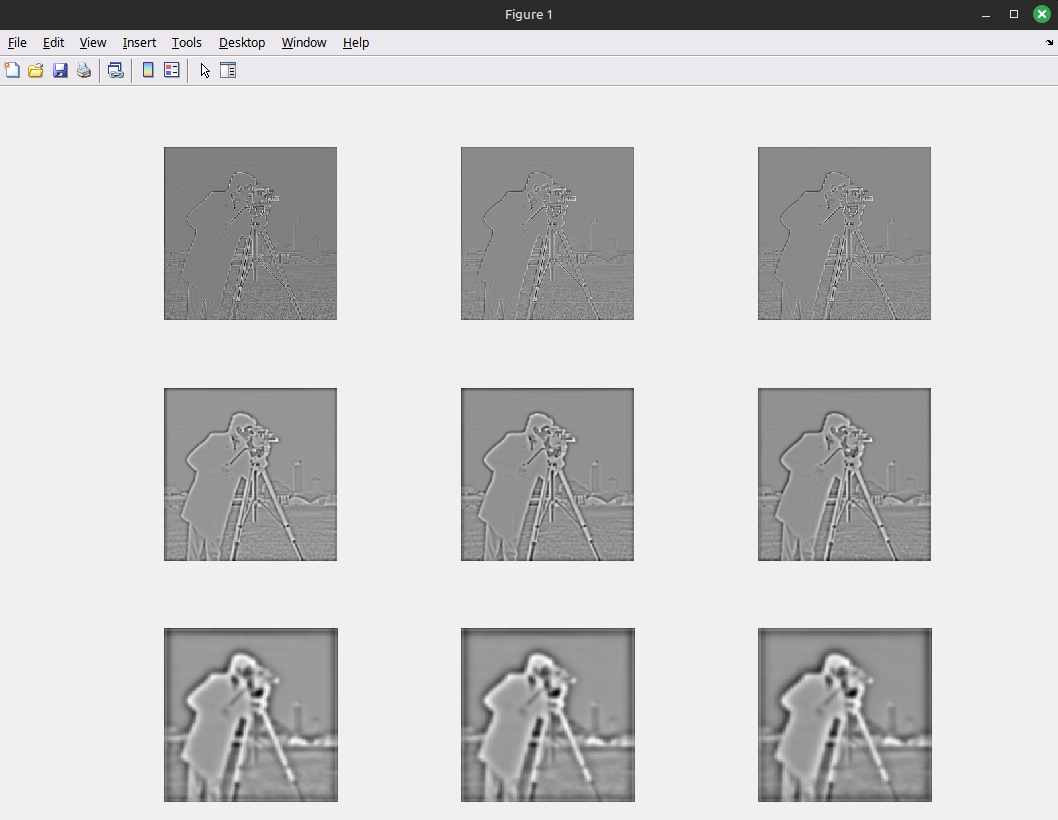
\includegraphics[width=0.5\textwidth]{DOG.png}
  \caption{DoG Pyramid}
  \end{figure}

\subsubsection{Plot 2 – Αρχική εικόνα \& candidate keypoints}
Αριστερά εμφανίζεται η αρχική εικόνα, ενώ δεξιά εμφανίζονται τα candidate keypoints με κόκκινους σταυρούς, όπου κάθε κόκκινος σταυρός αντιστοιχεί σε ένα τοπικό ακρότατο στο DoG. Υπάρχουν πολλοί κόκκινοι σταυροί σε όλη την εικόνα επειδή περιλαμβάνονται σημεία χαμηλής αντίθεσης και σημεία πάνω σε ακμές.
Αυτά τα keypoints είναι υποψήφια και εμφανίζονται πριν εφαρμοστεί το φιλτράρισμα για σταθερότητα και αντίθεση.
\begin{figure}[h!]
  \centering
  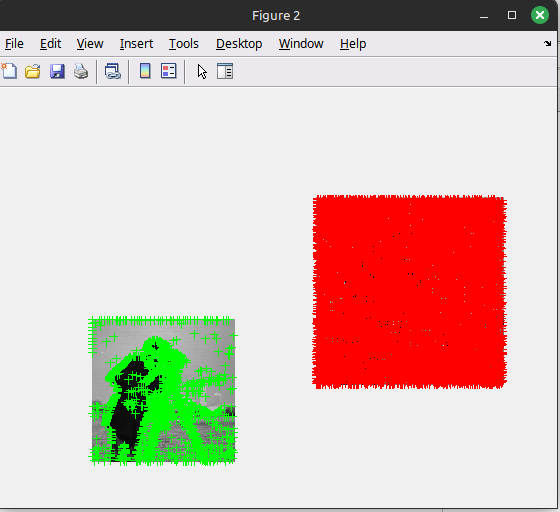
\includegraphics[width=0.55\textwidth]{RED.png}
  \caption{Αρχικά keypoints πριν το φιλτράρισμα}
  \end{figure}

\subsubsection{Plot 3 – Τελικά keypoints μετά το φιλτράρισμα}
Στα αριστερά εμφανίζονται πράσινοι σταυροί που υποδεικνύουν τα keypoints με αντίθεση πάνω από το προκαθορισμένο threshold,
ενώ τα keypoints χαμηλής αντίθεσης έχουν απορριφθεί. Αυτό οδηγεί σε σημαντική μείωση του πλήθους των σημάτων και αποφεύγονται τα σημεία
που είναι ευαίσθητα σε θόρυβο. \\

Στα δεξιά εμφανίζονται μπλε σταυροί που υποδεικνύουν τα keypoints που παραμένουν μετά τον έλεγχο edge responses. Διατηρούνται μόνο σταθερά γεωμετρικά σημεία, ενώ τα keypoints πάνω σε ευθείες απορρίπτονται.
Κάθε keypoint πλέον έχει assigned orientation και είναι έτοιμο για τον υπολογισμό του descriptor, με ακόμη λιγότερα, αλλά πιο αξιόπιστα keypoints.
\newpage
  \begin{figure}[h!]
    \centering
    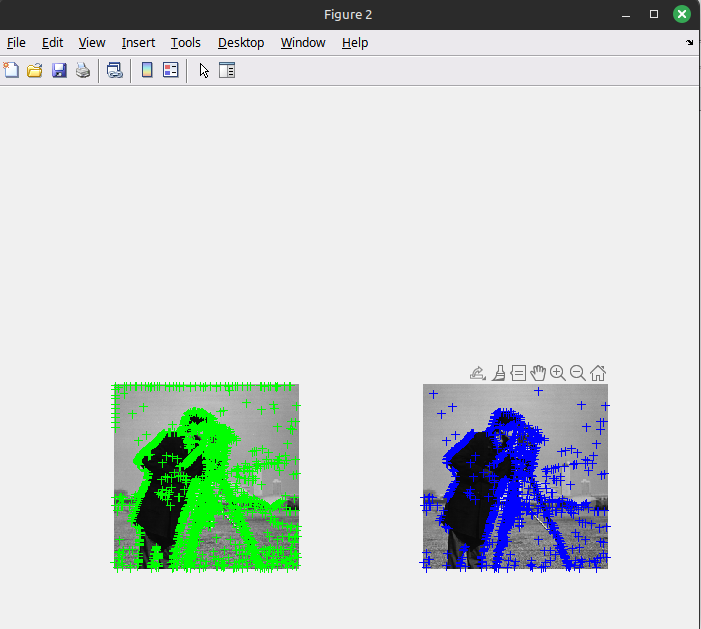
\includegraphics[width=0.6\textwidth]{BLUE.png}
    \caption{Keypoints μετά το φιλτράρισμα}
    \end{figure}


    \subsection{Αριθμός Επιπέδων Ανά Οκτάβα}
    Κάθε οκτάβα περιέχει εικόνες που έχουν φιλτραριστεί με gaussian blur σε διαφορετικά επίπεδα κλίμακας, τα οποία συμβολίζουμε με $s$.
    Το $s$ είναι ο αριθμός των επιπέδων DoG που θέλουμε να χρησιμοποιήσουμε για τον εντοπισμό ακροτάτων (\textit{extrema}) στο scale space. Κάθε DoG υπολογίζεται ως η διαφορά δύο συνεχόμενων gaussian εικόνων:
    
    \[
    \text{DoG}_i = G_{i+1} - G_i
    \]
    
    Για να εντοπιστούν τα \textit{extrema}, δεν χρησιμοποιούμε τα άκρα της οκτάβας, γιατί δεν έχουν γειτονικά επίπεδα πάνω ή κάτω για τον έλεγχο 3D ακροτάτων. Γι' αυτό χρειάζονται $s+2$ DoG εικόνες ώστε τα εσωτερικά DoG να καλύπτουν όλα τα $s$ επίπεδα.
    
    Κάθε DoG απαιτεί 2 gaussian εικόνες, άρα για $s+2$ DoG χρειαζόμαστε:
    
    \[
    \text{Gaussian images} = (\text{DoG count}) + 1 = (s+2) + 1 = s+3
    \]
    
    Τα $s+3$ Gaussian images εξασφαλίζουν σωστό έλεγχο 3D ακροτάτων και αποφεύγουν τα \textit{boundary errors}, δηλαδή σφάλματα στα άκρα της οκτάβας.
    
    
    \subsection{Εφαρμογή και Αποτελέσματα της Ανίχνευσης SIFT}
    Χρησιμοποιήθηκε υλοποίηση SIFT (\texttt{SIFT\_feature.m}) για την ανίχνευση keypoints σε πέντε grayscale εικόνες από τη βιβλιοθήκη του matlab.
    \subsubsection{Περιγραφή εικόνων}
    \begin{enumerate}
      \item \texttt{cameraman.tif} \\
      Γκρι εικόνα με άτομο σε πρώτο πλάνο. Παρουσιάζει πολλές ακμές και γωνίες (καθαρά όρια αντικειμένων), καλή αντίθεση και υφές(επαναλαμβανόμενα μοτίβα φωτεινότητας) στο φόντο.
  
      \item \texttt{coins.png} \\
      Γκρι εικόνα με κυκλικά αντικείμενα (νομίσματα). Έχει έντονα όρια, δηλαδή απότομη αλλαγή φωτεινότητας μεταξύ νομισμάτων και φόντου, και επαναλαμβανόμενα σχήματα.
  
      \item \texttt{pout.tif} \\
      Γκρι εικόνα προσώπου με χαμηλή αντίθεση, όπου η φωτεινότητα αλλάζει ομαλά. Κυριαρχούν μεγάλες ομοιόμορφες περιοχές χωρίς έντονες ακμές.
  
      \item \texttt{rice.png} \\
      Γκρι εικόνα με μικρούς φωτεινούς κόκκους σε σκούρο φόντο. Έχει υψηλή αντίθεση, γιατί οι κόκκοι ξεχωρίζουν καθαρά, και πολλές μικρές λεπτομέρειες.
  
      \item \texttt{moon.tif} \\
      Γκρι εικόνα με φυσικές υφές και κρατήρες. Περιέχει λεπτομέρειες μέσης κλίμακας και σχετικά ομαλές μεταβάσεις φωτεινότητας.
  \end{enumerate}
  
    
    \subsubsection{Αποτελέσματα SIFT}
    \begin{table}[h!]
      \centering
      \begin{tabular}{|l|c|}
      \hline
      \textbf{Εικόνα} & \textbf{Αριθμός Keypoints} \\
      \hline
      pout.tif & 30 \\
      coins.png & 1258 \\
      cameraman.tif & 1517 \\
      rice.png & 1701 \\
      moon.tif & 445 \\
      \hline
      \end{tabular}
      \caption{Αριθμός keypoints που εντοπίστηκαν σε κάθε εικόνα με τον αλγόριθμο \texttt{SIFT\_feature.m}}
      \end{table}
      
    
    \subsubsection{Σχολιασμός}
    Παρατηρείται σαφής συσχέτιση μεταξύ της υφής της εικόνας και του πλήθους των keypoints:

\begin{enumerate}
    \item Η εικόνα \texttt{rice.png} παρουσιάζει τον μεγαλύτερο αριθμό keypoints , λόγω της έντονης και πυκνής υφής της.
    \item Η \texttt{cameraman.tif} εμφανίζει επίσης μεγάλο αριθμό keypoints, καθώς περιέχει πολλές ακμές και δομές σε διαφορετικές κλίμακες.
    \item Η \texttt{coins.png} παρουσιάζει αρκετά keypoints κυρίως στα όρια των νομισμάτων.
    \item Η \texttt{moon.tif} έχει μέτριο αριθμό keypoints, οι οποίοι εντοπίζονται κυρίως στους κρατήρες και στα όρια του φόντου με το φεγγάρι.
    \item Η \texttt{pout.tif} εμφανίζει πολύ μικρό αριθμό keypoints, γεγονός που οφείλεται στο χαμηλό επίπεδο υφής και στις μεγάλες ομοιόμορφες περιοχές.
\end{enumerate}

    

\section{Υποκλιμακική Ακρίβεια}
Στον αλγόριθμο SIFT, τα πιθανά σημεία-κλειδιά βρίσκονται αρχικά ως τοπικά μέγιστα ή ελάχιστα της DoG στον διακριτό χώρο $(x,y,\sigma)$.
Αυτή η διακριτοποίηση δεν είναι ακριβής, γιατί τα πραγματικά ακρότατα της εικόνας δεν πέφτουν πάντα σε ακριβείς θέσεις ή κλίμακες.
Γι' αυτό γίνεται βελτίωση σε υποχωρικό και υποκλιμακικό επίπεδο, ώστε τα σημεία-κλειδιά να εντοπίζονται πιο σωστά και να είναι πιο σταθερά.

\subsection{Ανάπτυγμα Taylor της DoG στον Χώρο Κλίμακας}
Ουσιαστικά είναι η προσέγγιση της τιμής της DoG γύρω από ένα αρχικό ακρότατο με πολυώνυμο δεύτερης τάξης (2nd order Taylor expansion)
σε τρεις διαστάσεις $(x,y,\sigma)$:

\[
D(\mathbf{x}) \approx D + \nabla D^T \mathbf{x} + \frac{1}{2} \mathbf{x}^T H \mathbf{x}
\]

όπου:

\begin{itemize}
    \item $\mathbf{x} = (x,y,\sigma)^T$ είναι η μετατόπιση από τη διακριτή θέση του keypoint.
    \item $\nabla D$ είναι το διάνυσμα των πρώτων παραγώγων της DoG σε $x, y, \sigma$.
    \item $H$ είναι ο πίνακας Hessian, που περιέχει τις δεύτερες παραγώγους της DoG.
\end{itemize}


\paragraph{Υπολογισμός Ακρότατου}
\mbox{}\\

Η ακριβής θέση του ακρότατου υπολογίζεται με:

\[
\frac{\partial D}{\partial \mathbf{x}} = 0 \quad \Rightarrow \quad \hat{\mathbf{x}} = - H^{-1} \nabla D
\]

Αυτό το διάνυσμα $\hat{\mathbf{x}}$ δίνει την subpixel \& subscale θέση του keypoint.

\paragraph{Απόρριψη Ασταθών Keypoints}
\mbox{}\\

Η τιμή της DoG στο subscale ακρότατο είναι:

\[
D(\hat{\mathbf{x}}) = D + \frac{1}{2} \nabla D^T \hat{\mathbf{x}}
\]
Εάν η απόλυτη τιμή αυτής της DoG είναι μικρότερη από προκαθορισμένο κατώφλι, το keypoint απορρίπτεται. 
Αυτή η διαδικασία συνδέεται με τη θεωρία \textit{scale-space}: η DoG προσεγγίζει την κανονικοποιημένη λαπλασιανή, και η τιμή στο ακρότατο εκφράζει την καμπυλότητα της εικόνας στον χώρο κλίμακας.

\subsection{Παραβολική Παρεμβολή}
Μία άλλη μέθοδος είναι η παραβολική παρεμβολή είναι μια μέθοδος που χρησιμοποιείται για υπο-πίξελ και υπο-κλίμακα ακρίβεια στον εντοπισμό των keypoints.
Αντί να μένουμε στο πιο κοντινό pixel ή επίπεδο κλίμακας, η μέθοδος αυτή προσεγγίζει τη θέση της κορυφής (local maximum) με μια παραβολή.
Σε μία διάσταση, η θέση της κορυφής εκτιμάται με τον τύπο:

\[
x_{\text{peak}} = x_0 - \frac{f'(x_0)}{f''(x_0)}
\]

όπου:

\begin{itemize}
    \item $x_0$ = αρχική θέση (pixel ή επίπεδο)
    \item $f'(x_0)$ = πρώτη παράγωγος στο $x_0$
    \item $f''(x_0)$ = δεύτερη παράγωγος στο $x_0$
\end{itemize}

Η μέθοδος αυτή εφαρμόζεται ξεχωριστά στις τρεις διαστάσεις $(x,y,\sigma)$.


\subsection{Σύγκριση Μεθόδων}
\begin{table}[h!]
  \centering
  \begin{tabular}{|l|l|l|l|l|}
  \hline
  \textbf{Μέθοδος} & \textbf{Ακρίβεια} & \textbf{Κόστος} & \textbf{Σταθερότητα} & \textbf{SIFT} \\
  \hline
  Ανάπτυγμα Taylor & Υψηλή & Μεσαίο--Υψηλό & Πολύ Υψηλή & \ding{51} \\
  Παραβολική Παρεμβολή & Μεσαία & Χαμηλό & Περιορισμένη & \ding{55} \\
  \hline
  \end{tabular}
  \caption{Σύγκριση μεθόδων υποκλιμακικής εκτίμησης keypoints στον SIFT}
  \end{table}

Για ακριβή και σταθερά keypoints, το Taylor expansion είναι προτιμότερο, ενώ η παραβολική παρεμβολή είναι καλή σε περιπτώσεις που θέλουμε ταχύτητα.


\section{Αντιστοίχιση \& RANSAC}
Παρουσιάζεται η διαδικασία αντιστοίχισης των σημείων κλειδιών που εντοπίστηκαν με τον αλγόριθμο SIFT μεταξύ δύο εικόνων, καθώς και η εφαρμογή του αλγορίθμου
RANSAC για την απομάκρυνση των outliers και την εξαγωγή ενός γεωμετρικού μοντέλου μεταξύ των εικόνων.
\subsection{Ανάλυση του SIFT (sift.m)}
Σε αυτή την υποενότητα αναλύουμε τις τεχνικές που ενσωματώθηκαν  για τη μεγιστοποίηση της ακρίβειας.
\begin{enumerate}
  \item \textbf{Subpixel Localization \& Taylor Expansion: }Τα extrema στο
   DoG εντοπίζονται αρχικά σε διακριτό επίπεδο pixel. Για να βρούμε την πραγματική κορυφή ανάμεσα στα pixels, χρησιμοποιούμε ανάπτυγμα Taylor 2ης τάξης.
  \item \textbf{Edge Rejection (Hessian Matrix): } Για την απόρριψη σημείων κατά μήκος ακμών, υπολογίζεται ο πίνακας Hessian.
  \item \textbf{Trilinear Interpolation (Descriptor): }Η τιμή κάθε κλίσης (magnitude) παρεμβάλλεται σε τρεις διαστάσεις (θέση x,y και bin κατεύθυνσης),
   αυτό αποτρέπει απότομες αλλαγές στον περιγραφητή όταν το keypoint μετατοπίζεται ελάχιστα.
   \item \textbf{Gaussian Weighting \& Normalization: }
      \begin{itemize}
        \item Εφαρμόζεται ένα gaussian window στον περιγραφητή ώστε τα pixels μακριά από το κέντρο να έχουν μικρότερη βαρύτητα.
        \item Clipping (0.2): Έστω ότι τα στοιχεία του 128-διάστατου descriptor είναι 
        $\mathbf{v} = [v_1, v_2, \dots, v_{128}]$. 
        Εφαρμόζουμε \textit{clipping}:
        
        \[
        v_i \leftarrow \min(v_i, 0.2), \quad \forall i = 1, \dots, 128
        \]
        
        και στη συνέχεια κανονικοποιούμε ξανά τον descriptor:
        
        \[
        \mathbf{v} \leftarrow \frac{\mathbf{v}}{\|\mathbf{v}\|}, \quad \text{όπου} \quad \|\mathbf{v}\| = \sqrt{\sum_{i=1}^{128} v_i^2}.
        \]
        
        Αυτό εξασφαλίζει ότι ο descriptor παραμένει ανθεκτικός σε αλλαγές φωτεινότητας.
        
      \end{itemize}
\end{enumerate}



\subsection{Descriptor Matching (matching.m)}
Κάθε keypoint της εικόνας περιγράφεται από έναν 128-D SIFT descriptor, ο οποίος κωδικοποιεί την κατανομή των gradients στην τοπική περιοχή γύρω από το 
keypoint. 
Για την αντιστοίχιση μεταξύ δύο εικόνων, κάθε keypoint της εικόνας 1 συγκρίνεται με όλα τα keypoints της εικόνας 2 ώστε να βρεθεί το πιο παρόμοιο.

\subsubsection{Μέθοδοι υπολογισμού ομοιότητας }
\paragraph{Euclidean Distance}
\mbox{}\\
Η ευκλείδεια απόσταση μεταξύ δύο descriptors $f_1$ και $f_2$ δίνεται από:

\[
d = \sum_{i=1}^{128} (f_1(i) - f_2(i))^2
\]

Μικρότερη απόσταση σημαίνει μεγαλύτερη ομοιότητα.


\paragraph{Ratio Test }
\mbox{}\\

Υπολογίζονται οι δύο μικρότερες αποστάσεις $d_1$ και $d_2$ από όλα τα keypoints της δεύτερης εικόνας.
Διατηρούμε την αντιστοιχία μόνο αν ισχύει:

\[
\frac{d_1}{d_2} < 0.7
\]

Αυτό σημαίνει ότι η καλύτερη αντιστοιχία πρέπει να είναι καλύτερη από τη δεύτερη καλύτερη και γενικά η μέθοδος αυτή απομακρύνει λάθος αντιστοιχίσεις

\subsection{RANSAC}
Ακόμα και με το Ratio Test, πολλές αντιστοιχίσεις θα είναι λανθασμένες (outliers). Ο RANSAC (Random Sample Consensus) είναι ένας επαναληπτικός αλγόριθμος
που εκτιμά τις παραμέτρους ενός μαθηματικού μοντέλου (π.χ. affine transformation) από ένα σύνολο παρατηρήσεων που περιέχει θόρυβο.

\subsubsection{Χρήση του στο SIFT Matching}
Μετά την αρχική αντιστοίχιση των keypoints με βάση τους SIFT descriptors και το ratio test, έχουμε ένα σύνολο πιθανών αντιστοιχιών.
Κάποια από αυτά μπορεί να είναι λανθασμένα, λόγω επαναλαμβανόμενων μοτίβων, θορύβου ή αλλαγών στην προβολή της σκηνής.
\paragraph{Βήματα εφαρμογής RANSAC (rasnac.m)}
\mbox{}\\
\begin{enumerate}
  \item \textbf{Ελάχιστο Δείγμα: }
  Επιλέγονται τυχαία $n$ ζεύγη σημείων. Για την εκτίμηση ενός affine μετασχηματισμού
  απαιτούνται τουλάχιστον $n = 3$ σημεία, ώστε να προσδιοριστούν οι παράμετροι
  του μετασχηματισμού, δηλαδή η μετατόπιση, η περιστροφή, η κλιμάκωση και η στρέβλωση.
  
  \item \textbf{Model Estimation: } Ένα σημείο $(x, y)$ της πρώτης εικόνας μετασχηματίζεται στο σημείο $(x', y')$ 
  της δεύτερης εικόνας μέσω του πίνακα $M$:

  \[
  \begin{bmatrix}
  x' \\
  y'
  \end{bmatrix}
  =
  \begin{bmatrix}
  m_{11} & m_{12} \\
  m_{21} & m_{22}
  \end{bmatrix}
  \begin{bmatrix}
  x \\
  y
  \end{bmatrix}
  +
  \begin{bmatrix}
  t_x \\
  t_y
  \end{bmatrix}
  \]
  
  Για την επίλυση, ο RANSAC επιλέγει 3 τυχαία ζεύγη σημείων και λύνει το σύστημα:
  
  \[
  \mathbf{p}' = M \mathbf{p}
  \]
  
  όπου ο πίνακας $M$ υπολογίζεται με τη μέθοδο Least Squares πάνω στο τυχαίο δείγμα.
  

  \item \textbf{Υπολογισμός Σφάλματος: } Για να κριθεί αν μία αντιστοίχιση $i$ είναι \textbf{inlier}, υπολογίζεται η ευκλείδεια απόσταση:
  
  \[
  \varepsilon_i
  =
  (x'_i - \hat{x}'_i)^2 + (y'_i - \hat{y}'_i)^2
  \]
  
  Αν ισχύει $\varepsilon_i < \text{threshold}$ (π.χ. $5$ pixels), τότε η αντιστοίχιση θεωρείται έγκυρη.
  
  \item \textbf{Consensus: } Αν η απόσταση είναι μικρότερη από ένα max distance (π.χ. 5 pixels), το σημείο θεωρείται inlier.
  \item \textbf{Επαναλήψεις και επιλογή καλύτερου μοντέλου: }
  \begin{itemize}
      \item Το βήμα επαναλαμβάνεται για $N$ επαναλήψεις (π.χ., 2000).
      \item Κρατάμε το μοντέλο $M$ με τα περισσότερα inliers.
  \end{itemize}
\end{enumerate}

\subsection{Πειράματα Αποτελεσμάτων}
\begin{table}[h!]
  \centering
  \resizebox{0.98\textwidth}{!}{
  \small
  \begin{tabular}{|c|l|c|c|c|c|}
  \hline
  \textbf{Δοκιμή} & \textbf{Συνθήκη Μετασχηματισμού} & \textbf{Keypoints (Img 1 / 2)} & \textbf{Total Matches} & \textbf{RANSAC Inliers} & \textbf{Inlier Ratio} \\
  \hline
  1 & Rotation (15°) \& Scale (0.8) & 445 / 268 & 123 & 120 & 97.56\% \\
  2 & Rotation (45°) & 445 / 422 & 232 & 228 & 98.28\% \\
  3 & Scale (3.5) & 445 / 1866 & 184 & 178 & 96.74\% \\
  4 & Gaussian Noise (0.01) & 445 / 1042 & 126 & 124 & 98.41\% \\
  5 & Brightness (+50) & 445 / 441 & 410 & 410 & 100.00\% \\
  \hline
  \end{tabular}
  }
  \caption{Αποτελέσματα δοκιμών αντιστοίχισης keypoints με RANSAC}
  \end{table}


\subsubsection{Invariance στην Περιστροφή (Rotation 15\textdegree{} \& 45\textdegree{})}  
\paragraph{Αποτελέσματα : }Inlier Ratio 97.56\% και 98.28\%.
\mbox{}\\
\paragraph{Γιατί δουλεύει:}
\mbox{}\\
\begin{itemize}
  \item Ο SIFT υπολογίζει το ιστόγραμμα προσανατολισμού (orientation histogram) για κάθε keypoint.
  \item Η κυρίαρχη γωνία κάθε keypoint χρησιμοποιείται για να περιστραφεί ο περιγραφητής στη “κανονική” του μορφή (rotation normalization).
\end{itemize}

\paragraph{Γιατί όχι 100\%:}
\mbox{}\\
\begin{itemize}
  \item \textbf{Quantization: }Τα pixels είναι διακριτά (0–255 ή 0–1), οπότε μικρές μετατοπίσεις δημιουργούν στρογγυλοποιήσεις.
  \item \textbf{Interpolation Artifacts: }Όταν περιστρέφουμε μια ψηφιακή εικόνα, τα pixels δεν πέφτουν ακριβώς πάνω στο αρχικό πλέγμα, οπότε οι τιμές τους υπολογίζονται μέσω παρεμβολής. 
  Αυτή η διαδικασία αλλάζει ελαφρώς τις τιμές των pixels και συνεπώς τους gradients, με αποτέλεσμα κάποιοι keypoints να διαφοροποιούνται.
\end{itemize}


\subsubsection{Invariance στην Κλίμακα (Scale 3.5)}
\paragraph{Αποτελέσματα : }Inlier Ratio 96.74\%.
\mbox{}\\


\paragraph{Γιατί δουλεύει:}
\mbox{}\\
\begin{itemize}
  \item Ο SIFT δημιουργεί μια gaussian \& DoG πυραμίδα σε πολλές κλίμακες.
  \item Keypoints ανιχνεύονται ως extrema σε πολλαπλές οκτάβες, οπότε αν μια λεπτομέρεια είναι μικρή ή μεγάλη, εξακολουθεί να αναγνωρίζεται.
\end{itemize}


\paragraph{Γιατί όχι 100\%:}
\mbox{}\\
\begin{itemize}
  \item \textbf{Απώλεια πληροφορίας: }Όταν μεγαλώνουμε μια εικόνα, γίνεται interpolation, δηλαδή προσθέτουμε νέα pixel values που δεν υπήρχαν.
  \item Όταν μικραίνουμε, χάνεται λεπτομέρεια.
  \item \textbf{Subpixel Localization: }Χρησιμοποιεί Taylor expansion, δηλαδή μια προσέγγιση, που μπορεί να δώσει ελαφρώς διαφορετικές συντεταγμένες.
\end{itemize}


\subsubsection{Invariance στον Φωτισμό (Brightness +50)}
\paragraph{Αποτελέσματα : }Inlier Ratio 100.00\%.
\mbox{}\\


\paragraph{Γιατί δουλεύει:}
\mbox{}\\
\begin{itemize}
  \item Ο SIFT βασίζεται σε gradients, δηλαδή διαφορές μεταξύ γειτονικών pixels, που είναι ανεξάρτητες από ομοιόμορφη αύξηση φωτεινότητας.
  \item \textbf{Descriptor Normalization} ($\|v\| = 1$) καθιστά τις τιμές των gradients σχετικές και όχι απόλυτες, διασφαλίζοντας ότι η συνολική τους ένταση είναι 1.
\end{itemize}


\subsubsection{Αντοχή στον Θόρυβο (Gaussian Noise 0.01)}
\paragraph{Αποτελέσματα : }Inlier Ratio 98.41\%.
\mbox{}\\

\paragraph{Γιατί δουλεύει:}
\mbox{}\\
\begin{itemize}
  \item Ο SIFT εφαρμόζει gaussian blur πριν την εξαγωγή των χαρακτηριστικών, που λειτουργεί σαν φίλτρο και μειώνει τον θόρυβο.
  \item Το RANSAC απορρίπτει τα περισσότερα λανθασμένα extrema που δημιουργεί ο θόρυβος, κρατώντας μόνο τα αληθινά keypoints.
\end{itemize}

\paragraph{Γιατί όχι 100\%:}
\mbox{}\\
\begin{itemize}
  \item Όταν προσθέτουμε θόρυβο, δημιουργούνται νέα τοπικά maxima/minima (extrema),
   κάποια από τα οποία δεν αντιστοιχούν σε πραγματικές λεπτομέρειες της εικόνας.
  \item Μερικά keypoints αλλάζουν ελαφρά θέση ή orientation λόγω του θορύβου, μειώνοντας ελαφρά τον αριθμό των inliers.
\end{itemize}


\section{Σύγκριση \& Πολυπλοκότητα}
Εξετάζουμε τη σύγκριση και την υπολογιστική πολυπλοκότητα των αλγορίθμων ανίχνευσης και περιγραφής τοπικών χαρακτηριστικών εικόνας, όπως οι SIFT, GLOH και SURF, αναλύοντας τα πλεονεκτήματα,
τις αδυναμίες τους και το κόστος εκτέλεσής τους σε σχέση με την αποτελεσματικότητα στην αναγνώριση και αντιστοίχιση χαρακτηριστικών.
\subsection{SIFT vs GLOH vs SURF}
Αυτές οι μέθοδοι είναι local feature descriptors,
δηλαδή τρόποι να περιγράψουμε τα keypoints μιας εικόνας για σύγκριση, αναγνώριση ή αντιστοίχιση.
\subsubsection{SIFT (Scale-Invariant Feature Transform)}
Ανίχνευση και περιγραφή χαρακτηριστικών ανεξάρτητα από κλίμακα, περιστροφή ή φωτεινότητα.
\paragraph{Βασικά βήματα:}
\mbox{}\\
\begin{enumerate}
  \item \textbf{Detection of extrema:}
  \begin{itemize}
      \item Υπολογισμός DoG:
      \[
      D(x,y,\sigma) = L(x,y,k\sigma) - L(x,y,\sigma)
      \]
      όπου $L(x,y,\sigma)$ είναι η εικόνα με Gaussian blur.
  \end{itemize}
  
  \item \textbf{Keypoint localization:}
  \begin{itemize}
      \item Ακριβής προσδιορισμός θέσεων και απόρριψη ασταθών ή χαμηλής αντίθεσης keypoints.
  \end{itemize}
  
  \item \textbf{Orientation assignment:}
  \begin{itemize}
      \item Ανάθεση κατεύθυνσης στο keypoint για ανθεκτικότητα σε περιστροφές.
  \end{itemize}
  
  \item \textbf{Descriptor computation:}
  \begin{itemize}
      \item Δημιουργία 128-D διανύσματος από orientation histograms.
  \end{itemize}
\end{enumerate}

\paragraph{Πλεονεκτήματα}
\mbox{}\\
\begin{itemize}
  \item \textbf{Υψηλή ανθεκτικότητα σε αλλαγές κλίμακας και περιστροφής:} Προκύπτει γιατί χρησιμοποιείται DoG pyramid για διαφορετικές κλίμακες και οι προσανατολισμοί των histograms είναι ανεξάρτητοι από την περιστροφή.
  \item \textbf{Ανθεκτικό σε αλλαγές φωτεινότητας:} Ο SIFT χρησιμοποιεί normalized gradient magnitudes, άρα μικρές αλλαγές στην ένταση δε αλλοιώνουν τους descriptors.
  \item \textbf{Ακριβές matching:} Τα 128 στοιχεία του descriptor περιγράφουν το περιβάλλον του keypoint.
\end{itemize}


\paragraph{Μειονεκτήματα}
\mbox{}\\
\begin{itemize}
  \item \textbf{Υψηλή υπολογιστική πολυπλοκότητα:} Ο DoG σε πολλαπλές κλίμακες και η κατασκευή των 128-διάστατων histograms απαιτούν μεγάλο αριθμό υπολογισμών . 
  \item \textbf{Αργή εκτέλεση σε μεγάλες εικόνες:} Πολλά keypoints και μεγάλες εικόνες αυξάνουν γραμμικά τον χρόνο.
  \item \textbf{Μεγάλη χρήση μνήμης:} Κάθε keypoint έχει 128 αριθμούς floating point.
\end{itemize}


\subsubsection{GLOH (Gradient Location and Orientation Histogram)}
Βελτιωμένος SIFT descriptor

\paragraph{Βασικά βήματα:}
\mbox{}\\
\begin{enumerate}
  \item Χωρίζει την περιοχή γύρω από το keypoint σε \textit{log-polar grid} (ένα πλέγμα που χωρίζει την περιοχή σε κυκλικά και ακτινικά τμήματα αντί για απλά τετράγωνα $4\times4$).
  \item Ο αρχικός descriptor έχει 272 διαστάσεις και μειώνεται σε 128 μέσω PCA. 
  \item Βασίζεται στην ίδια ανίχνευση keypoints όπως ο SIFT.
\end{enumerate}

\paragraph{Πλεονεκτήματα}
\mbox{}\\
\begin{itemize}
  \item \textbf{Καλύτερη διάκριση:} Το log-polar grid καταγράφει περισσότερες λεπτομέρειες στις περιοχές κοντά στο keypoint.  
  \item \textbf{Περισσότερο ανθεκτικό σε περιστροφές και μικρές παραμορφώσεις:} Η κυκλική και ακτινική διάταξη του grid μειώνει τις παραμορφώσεις, καθώς οι αλλαγές θέσης ή κλίσης των pixels επηρεάζουν λιγότερο τα συνολικά τμήματα. 
  \item \textbf{Ιδανικό για εφαρμογές με υψηλή ακρίβεια:} Το μεγάλο αρχικό descriptor καταγράφει περισσότερη πληροφορία.
\end{itemize}




\paragraph{Μειονεκτήματα}
\mbox{}\\
\begin{itemize}
  \item \textbf{Πιο αργό από SIFT:} Περισσότεροι υπολογισμοί ανά keypoint (272 στοιχεία αντί 128). 
  \item \textbf{Απαιτεί PCA για μείωση διαστάσεων:} Διαφορετικά, η μνήμη και ο χρόνος matching αυξάνονται σημαντικά. 
  \item \textbf{Πολύπλοκη υλοποίηση:} Το log-polar grid απαιτεί περισσότερους υπολογισμούς για κάθε keypoint.
\end{itemize}


\subsubsection{SURF (Speeded-Up Robust Features)}
Γρήγορος descriptor για real time εφαρμογές.


\paragraph{Βασικά βήματα:}
\mbox{}\\
\begin{enumerate}
  \item \textbf{Keypoint detection:}
  \begin{itemize}
      \item Χρησιμοποιείται Hessian matrix
      \[
      H(x,\sigma) = 
      \begin{bmatrix}
      L_{xx} & L_{xy} \\
      L_{xy} & L_{yy}
      \end{bmatrix}
      \]
      όπου $L_{xx}, L_{xy}, L_{yy}$ είναι οι δεύτερες παράγωγοι της εικόνας μετά από gaussian φίλτρο κλίμακας $\sigma$.
      \item Για γρήγορο υπολογισμό χρησιμοποιούνται τα \textit{integral images}, δηλαδή εικόνα όπου κάθε σημείο αποθηκεύει το άθροισμα όλων των pixel από την πάνω αριστερή γωνία μέχρι εκείνο το σημείο, ώστε να υπολογίζονται γρήγορα τα αθροίσματα τμημάτων της εικόνας.
  \end{itemize}
  
  \item \textbf{Descriptor computation:}
  \begin{itemize}
      \item Ο descriptor έχει 64 διαστάσεις και υπολογίζεται από Haar wavelets, δηλαδή απλά φίλτρα που μετρούν τις διαφορές έντασης σε οριζόντια και κατακόρυφα μοτίβα.
      \item Η περιοχή γύρω από το keypoint χωρίζεται σε μικρά τετράγωνα.
      \item Σε κάθε υπο-περιοχή υπολογίζονται οι αθροιστικές αποκρίσεις Haar wavelets σε $x$ και $y$ κατεύθυνση, δημιουργώντας γρήγορα υπολογιζόμενο descriptor.
  \end{itemize}
\end{enumerate}



\paragraph{Πλεονεκτήματα}
\mbox{}\\
\begin{itemize}
  \item \textbf{Γρήγορο:} Integral images επιτρέπουν υπολογισμούς περιοχών σε σταθερό χρόνο, μειώνοντας τον αριθμό των operations.
  
  \item \textbf{Καλή ανθεκτικότητα σε φωτεινότητα:} Όπως SIFT, χρησιμοποιεί gradients.
  
  \item \textbf{Μικρή χρήση μνήμης:} 64-διάστατος descriptor αντί 128, λιγότερη αποθήκευση.
\end{itemize}



\paragraph{Μειονεκτήματα}
\mbox{}\\
\begin{itemize}
  \item \textbf{Λιγότερο ανθεκτικό σε μεγάλες περιστροφές ή αλλαγές κλίμακας:} Η χρήση box filters αποτυπώνει γενικά μοτίβα φωτεινότητας και όχι λεπτομέρειες, οπότε η αναγνώριση δυσκολεύει όταν η εικόνα περιστρέφεται ή αλλάζει μέγεθος. 
  \item \textbf{Λιγότερη ακρίβεια σε πολύπλοκες σκηνές:} Ο μικρότερος descriptor χάνει σημαντικές λεπτομέρειες, με αποτέλεσμα να μειώνεται η ακρίβεια σε εικόνες με πολλαπλά αντικείμενα ή πολύπλοκες υφές.
\end{itemize}

\subsection{Υπολογιστικό κόστος}
Το υπολογιστικό κόστος εξαρτάται από δύο κύρια στάδια: keypoint detection και descriptor computation.

\subsubsection{SIFT}
\begin{enumerate}
  \item \textbf{Keypoint Detection -- DoG Pyramid}
  \begin{itemize}
      \item Ο SIFT ανιχνεύει keypoints κατασκευάζοντας μια πυραμίδα κλίμακας με DoG.
      \item Η διαδικασία περιλαμβάνει:
      \begin{itemize}
          \item υπολογισμό gaussian blur σε κάθε κλίμακα,
          \item αφαίρεση διαδοχικών gaussian εικόνων για την παραγωγή DoG,
          \item έλεγχο τοπικών ακροτάτων σε χώρο και κλίμακα.
      \end{itemize}
      \item Για εικόνα διαστάσεων $N \times N$ και $S$ κλίμακες:
      \begin{itemize}
          \item κάθε γκαουσιανή συνέλιξη έχει κόστος $O(N^2)$,
          \item για $S$ κλίμακες το συνολικό κόστος είναι $O(S \cdot N^2)$.
      \end{itemize}
      \item Το στάδιο αυτό είναι το πιο υπολογιστικά απαιτητικό και κυριαρχεί στον συνολικό χρόνο εκτέλεσης.
  \end{itemize}

  \item \textbf{Descriptor Computation}
  \begin{itemize}
      \item Για κάθε ένα από τα $K$ keypoints:
      \begin{itemize}
          \item αναλύεται ένα τοπικό patch $16 \times 16$ pixel,
          \item υπολογίζονται οι προσανατολισμοί κλίσης,
          \item παράγεται descriptor 128 διαστάσεων.
      \end{itemize}
      \item Το κόστος ανά keypoint είναι σταθερό, καθώς το μέγεθος του patch και ο αριθμός των bins είναι προκαθορισμένα.
      \item Συνεπώς, το συνολικό κόστος του σταδίου είναι $O(K)$.
  \end{itemize}

  \item \textbf{Συνολικό Κόστος SIFT}
  \[
      O(S \cdot N^2 + K)
  \]
  Η πλειονότητα του χρόνου εκτέλεσης δαπανάται στη δημιουργία της DoG πυραμίδας, ιδιαίτερα για εικόνες υψηλής ανάλυσης.
\end{enumerate}

\subsubsection{GLOH}
\begin{enumerate}
    \item \textbf{Keypoint Detection}
    \begin{itemize}
        \item Ίδιος μηχανισμός με τον SIFT (DoG pyramid).
        \item Κόστος: $O(S \cdot N^2)$
    \end{itemize}

    \item \textbf{Descriptor Computation}
    \begin{itemize}
        \item Χρησιμοποιεί log-polar grid.
        \item Παράγει αρχικό descriptor 272 διαστάσεων.
        \item Εφαρμόζεται PCA για μείωση σε 128 διαστάσεις.
        \item Κόστος μεγαλύτερο από SIFT λόγω πυκνότερου grid και PCA.
    \end{itemize}
\end{enumerate}

\subsubsection{SURF}
\begin{enumerate}
    \item \textbf{Integral Images}
    \begin{itemize}
        \item Κάθε pixel περιέχει άθροισμα όλων των pixels πάνω και αριστερά του.
        \item Υπολογίζεται μία φορά με κόστος $O(N^2)$.
        \item Επιτρέπει υπολογισμό αθροισμάτων σε οποιοδήποτε ορθογώνιο τμήμα σε χρόνο $O(1)$.
    \end{itemize}

    \item \textbf{Box Filters \& Haar Wavelets}
    \begin{itemize}
        \item Box filters για γρήγορη προσέγγιση Gaussian φίλτρων.
        \item Haar wavelets μετρούν διαφορές έντασης μεταξύ γειτονικών περιοχών.
        \item Χάρη στις integral images, υπολογίζονται με λίγες πράξεις.
    \end{itemize}

    \item \textbf{Keypoint Detection}
    \begin{itemize}
        \item Εξετάζονται $S$ κλίμακες.
        \item Θεωρητικό κόστος $O(S \cdot N^2)$.
        \item Στην πράξη, τα box filters κάνουν τον SURF πιο γρήγορο από τον SIFT.
    \end{itemize}

    \item \textbf{Descriptor Computation}
    \begin{itemize}
        \item Descriptor 64 διαστάσεων.
        \item Υπολογίζεται σε patch σταθερού μεγέθους.
        \item Κόστος ανά keypoint σταθερό → συνολικά $O(K)$.
    \end{itemize}

    \item \textbf{Συνολικό Κόστος SURF}
    \begin{itemize}
        \item Χάρη σε integral images, box filters και μικρότερο descriptor, ο SURF έχει χαμηλότερο υπολογιστικό κόστος.
    \end{itemize}
\end{enumerate}


\subsection{Σύγκριση Αλγορίθμων}
\begin{table}[h!]
\begin{flushright}
\resizebox{0.95\textwidth}{!}{
\begin{tabular}{|l|c|p{3.5cm}|c|p{3.5cm}|p{2cm}|}
\hline
\textbf{Μέθοδος} & \textbf{Descriptor} & \textbf{Ανθεκτικότητα} & \textbf{Ταχύτητα} & \textbf{Κόστος} & \textbf{Επιλογή} \\
\hline
SIFT & 128 & Υψηλή (κλίμακα, περιστροφή και φωτεινότητα) & Αργή & Υψηλό λόγω DoG pyramid σε πολλές κλίμακες και μεγάλου descriptor & Ακρίβεια \\
\hline
GLOH & 128 (μετά PCA) & Πολύ υψηλή, (καλύτερη διάκριση χαρακτηριστικών) & Πολύ αργή & Πολύ υψηλό - log polar grid, descriptor 272 διαστάσεων \& PCA & Υψηλή ακρίβεια \\
\hline
SURF & 64 & Καλή (φωτεινότητα και μικρές περιστροφές, λιγότερο σε μεγάλες αλλαγές κλίμακας) & Γρήγορη & Χαμηλό χάρη σε integral images, box filters και μικρό descriptor & Ταχύτητα \\
\hline
\end{tabular}
}
\caption{Σύγκριση SIFT - GLOH - SURF}
\end{flushright}
\end{table}
















\end{document}